\documentclass[9pt,twocolumn]{article}
\usepackage{mathptmx} % Times font with math support
\usepackage{amsmath}
\usepackage{amssymb}
\usepackage{graphicx}
\usepackage{xcolor}
\usepackage{hyperref}
\usepackage{lipsum} % For dummy text, you can remove this line
\usepackage{subcaption}
\usepackage{booktabs}
% Set the paper margins
\usepackage[margin=1in]{geometry}
\usepackage{adjustbox}
% Set the line spacing
\renewcommand{\baselinestretch}{1.1}

% Set the title and authors
\title{\textbf{\textsc{Unsupervised learning - Anomaly detection}}}
\author{
  \textbf{Mirko Morello} \\
  $920601$ \\
  m.morello11@campus.unimib.it \\
  \and
  \textbf{Andrea Borghesi} \\
    $916202$ \\
  a.borghesi1@campus.unimib.it
}

% Customize section headings
\usepackage{titlesec}
\titleformat{\section}{\large\bfseries\scshape\color{black}}{\thesection}{1em}{}
\titleformat{\subsection}{\bfseries}{\thesubsection}{1em}{}
\begin{document}

\twocolumn[
  \begin{@twocolumnfalse}
    \maketitle
  \end{@twocolumnfalse}
]

% Introduction
\section{Introduction}

 % \begin{figure}[h]
 %     \centering
 %     \includegraphics[width=0.2\textwidth]{images/transformer-encoder.png}
 %     \caption{Transformer encoder architecture}
 %     \label{fig:transformer-encoder}
 % \end{figure}
Anomaly detection plays a crucial role in various domains, including fraud detection, network intrusion detection, and medical diagnosis. Anomalies, being rare and significantly different from the norm, can have critical implications. However, detecting anomalies poses several challenges, such as the scarcity of labeled anomalous data, the need for unsupervised methods, and the high dimensionality of datasets.
This report focuses on exploring unsupervised anomaly detection techniques applied to a high-dimensional medical dataset containing a mix of numerical and categorical features. We investigate several categories of anomaly detection methods, including proximity-based approaches, prototype-based methods, and reconstruction-based techniques.

\section{Dataset}
\subsection{Overview}
The available dataset is a medical dataset containing observations about patients. It comprises 7,200 observations, each with 23 dimensions or features. However, the labels or target variables were not provided, allowing only speculative analysis of the data's nature. The dataset consists of a mix of numerical and categorical features, where the categorical features have already been one-hot encoded.
The mixed nature of the data allowed for several observation discussed in the following sections.
\subsection{Data cleaning}
The dataset is presented with two features being empty for each data object, and therefore dropped them, remaining with 21 total features. The numerical features, initially saved as strings, had to be converted to \texttt{float64} values and then standardized with a Z-score, bringing the mean and standard deviation to $0$ and $1$ respectively.
Similarly, the apparent boolean futures were saved as string, therefore a cast to boolean has been necessary.\\
Other than these manipulation, the dataset did not present any other criticality, allowing us to proceed with our tasks.

\subsection{Data exploration}
Given the high dimensionality of the dataset, with 21 features, we implemented a couple of utility functions to facilitate approximate visualization of the data. The first method involved the use of dimensionality reduction algorithms, namely Principal Component Analysis (PCA) and t-Distributed Stochastic Neighbor Embedding (t-SNE), which allowed us to reduce the dimensionality while minimizing information loss.
Another useful visualization tool we developed involved plotting all combinations of numerical features to examine their relationships. These visualization tools played a crucial role, providing feedback and validation for our anomaly detection efforts.

\section{Proximity matrix for mixed data}
Due to the mixed nature of the dataset, consisting of both numerical and categorical features, a single global distance metric would not accurately capture the dissimilarity between observations across all features. To address this issue, we implemented a custom computation of the proximity matrix using Gower's distance metric, which combines multiple distance measures, providing a suitable dissimilarity measure for mixed data types. Specifically, for our task, the Euclidean distance was used for numerical features, and the Hamming distance was employed for categorical features. The resulting proximity matrix can be seen in Figure \ref{fig:proxmat}

\begin{figure}[h]
    \centering
    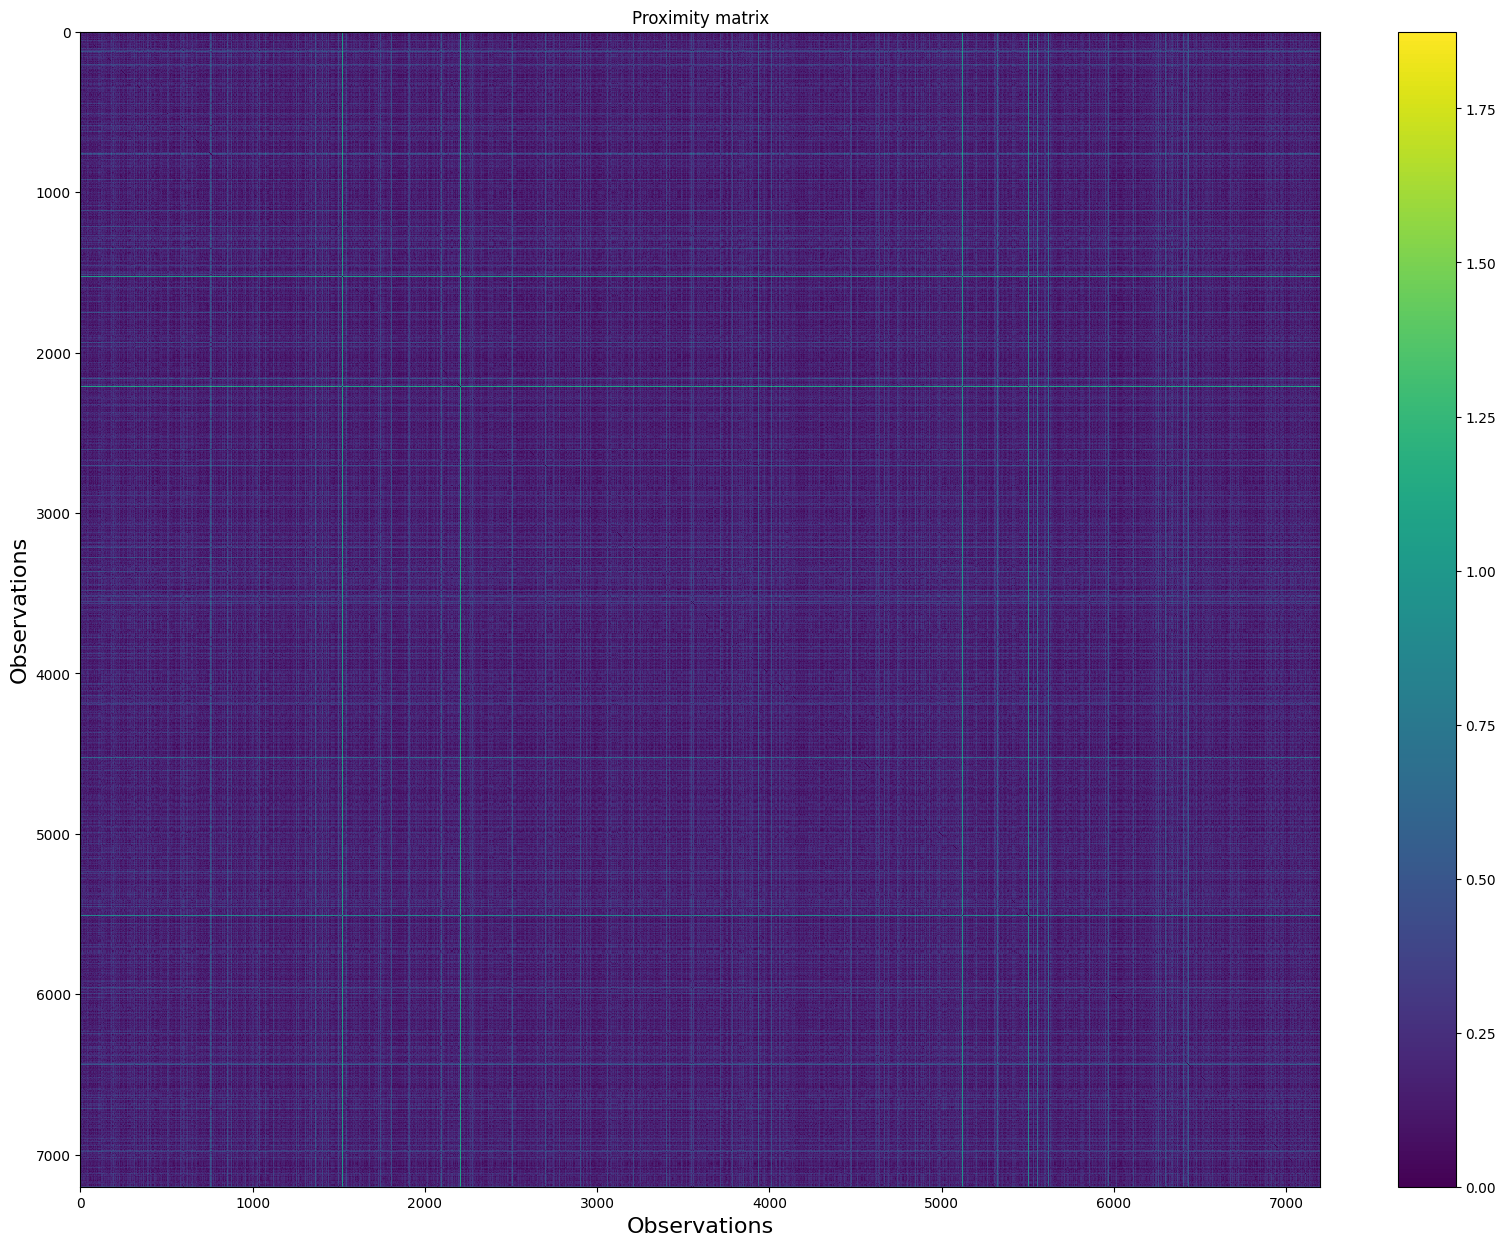
\includegraphics[width=0.5\textwidth]{images/proxmat.png}
    \caption{Proximity matrix of the data computed with Gower distance.}
    \label{fig:proxmat}
 \end{figure}

While our Python implementation of Gower's distance computation may not be as efficient as those found in other libraries, the proximity matrix calculation for the entire dataset took approximately 1.5 hours on a high-end consumer processor, despite the computational complexity. Given the large number of data objects, this duration can be considered feasible. To avoid unnecessary re-computations in subsequent runs, the proximity matrix has been saved to disk for future use.

\section{Thresholding anomaly scores}
Before delving into anomaly detection, we have to first decide where to put a threshold on the anomaly score that each method (aside from DBSCAN) will provide. There are several approaches in literature based on many statistics, we tried several of them and settled on the interquartile range (IQR).

The general approach with IQR thresholding defines a lower bound $T_{min}$ and an upper bound $T_{max}$ as
\begin{equation}
\begin{cases}
T_{min} = \mathrm{Q1} - c \cdot \mathrm{IQR} \\
T_{max} = \mathrm{Q3} + c \cdot \mathrm{IQR}
\end{cases}
\end{equation}
We set $c=1.5$, as it is, along with $c=2$, one of the most popular settings.
Unfortunately these statistic can be biased by the presence of the anomalies within the data when computed. Making the their use more inaccurate, therefore a two-stage approach is used to overcome this problem \cite{Yang2019OutlierDH}. We apply this threshold once to exclude the most obvious outliers, we recompute the bounds without the excluded data objects, and perform a second exclusion with the newly computed bounds. Since the anomaly scores that we will identify an anomaly when such score is high, we will apply the upper bound only.

\section{Proximity-based\\ anomaly detection}
The key assumption in proximity-based approaches for anomaly detection leverages spatial locality. Normal data objects are close to their neighbours, while anomalies are far from other data objects. Therefore, the general approach consists of evaluating the neighborhood of each data object to determine if it is anomalous or not. We can divide these approaches into two main areas: distance-based and density-based approaches. The former defines anomalies as data objects that are distant from other data objects, while the latter defines anomalies as data objects that reside in low-density regions.

\subsection{Distance-based anomaly detection with\\k-Nearest Neighbour}
The k-Nearest Neighbor (k-NN) algorithm for distance-based anomaly detection relies on the principle that anomalous data objects exhibit significantly larger distances to their k-nearest neighbors compared to ordinary data objects. By exploiting this property, the algorithm can effectively identify anomalies within the dataset.\\
To apply this approach, we computed the distance between each data object and its fifth nearest neighbour. The histogram of the distances of the points to their fifth nearest neighbour (Figure \ref{fig:nn_disthist}) shows how such measure is can be used as a proper anomaly score.
\begin{figure}[h]
    \centering
    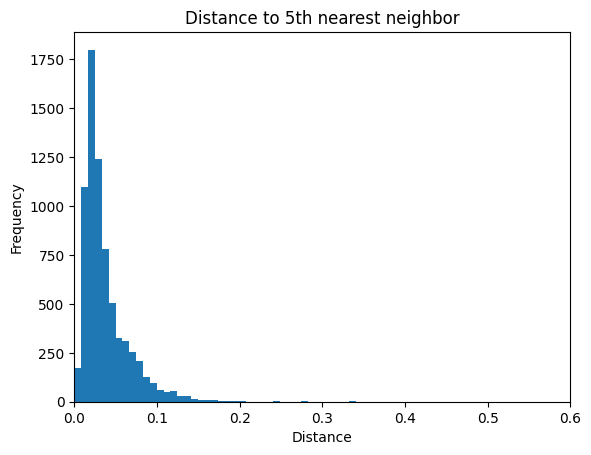
\includegraphics[width=0.5\textwidth]{images/NN_disthist.png}
    \caption{Histogram of the distances of each data object to its fifth nearest neighbour.}
    \label{fig:nn_disthist}
 \end{figure}
 
The application of this distance-based anomaly detection technique provided encouraging results, with visually distinct separation between anomalies and ordinary data objects as shown in Figure \ref{fig:nn_PCATSNE} and \ref{fig:nn_alldims}. The threshold derived from the two-step IQR thresholding resulted in the identification of 464 anomalies, constituting a reasonable 6.44\% of the entire dataset.

\begin{figure}[h]
    \centering
    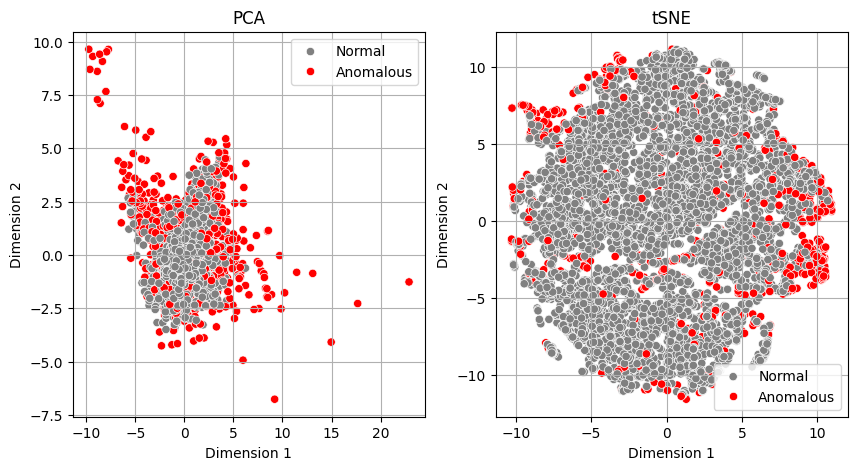
\includegraphics[width=0.5\textwidth]{images/NN_PCATSNE.png}
    \caption{Visual inspection of NN results on data reduced to two components.}
    \label{fig:nn_PCATSNE}
 \end{figure}


 \begin{figure*}[h]
    \centering
    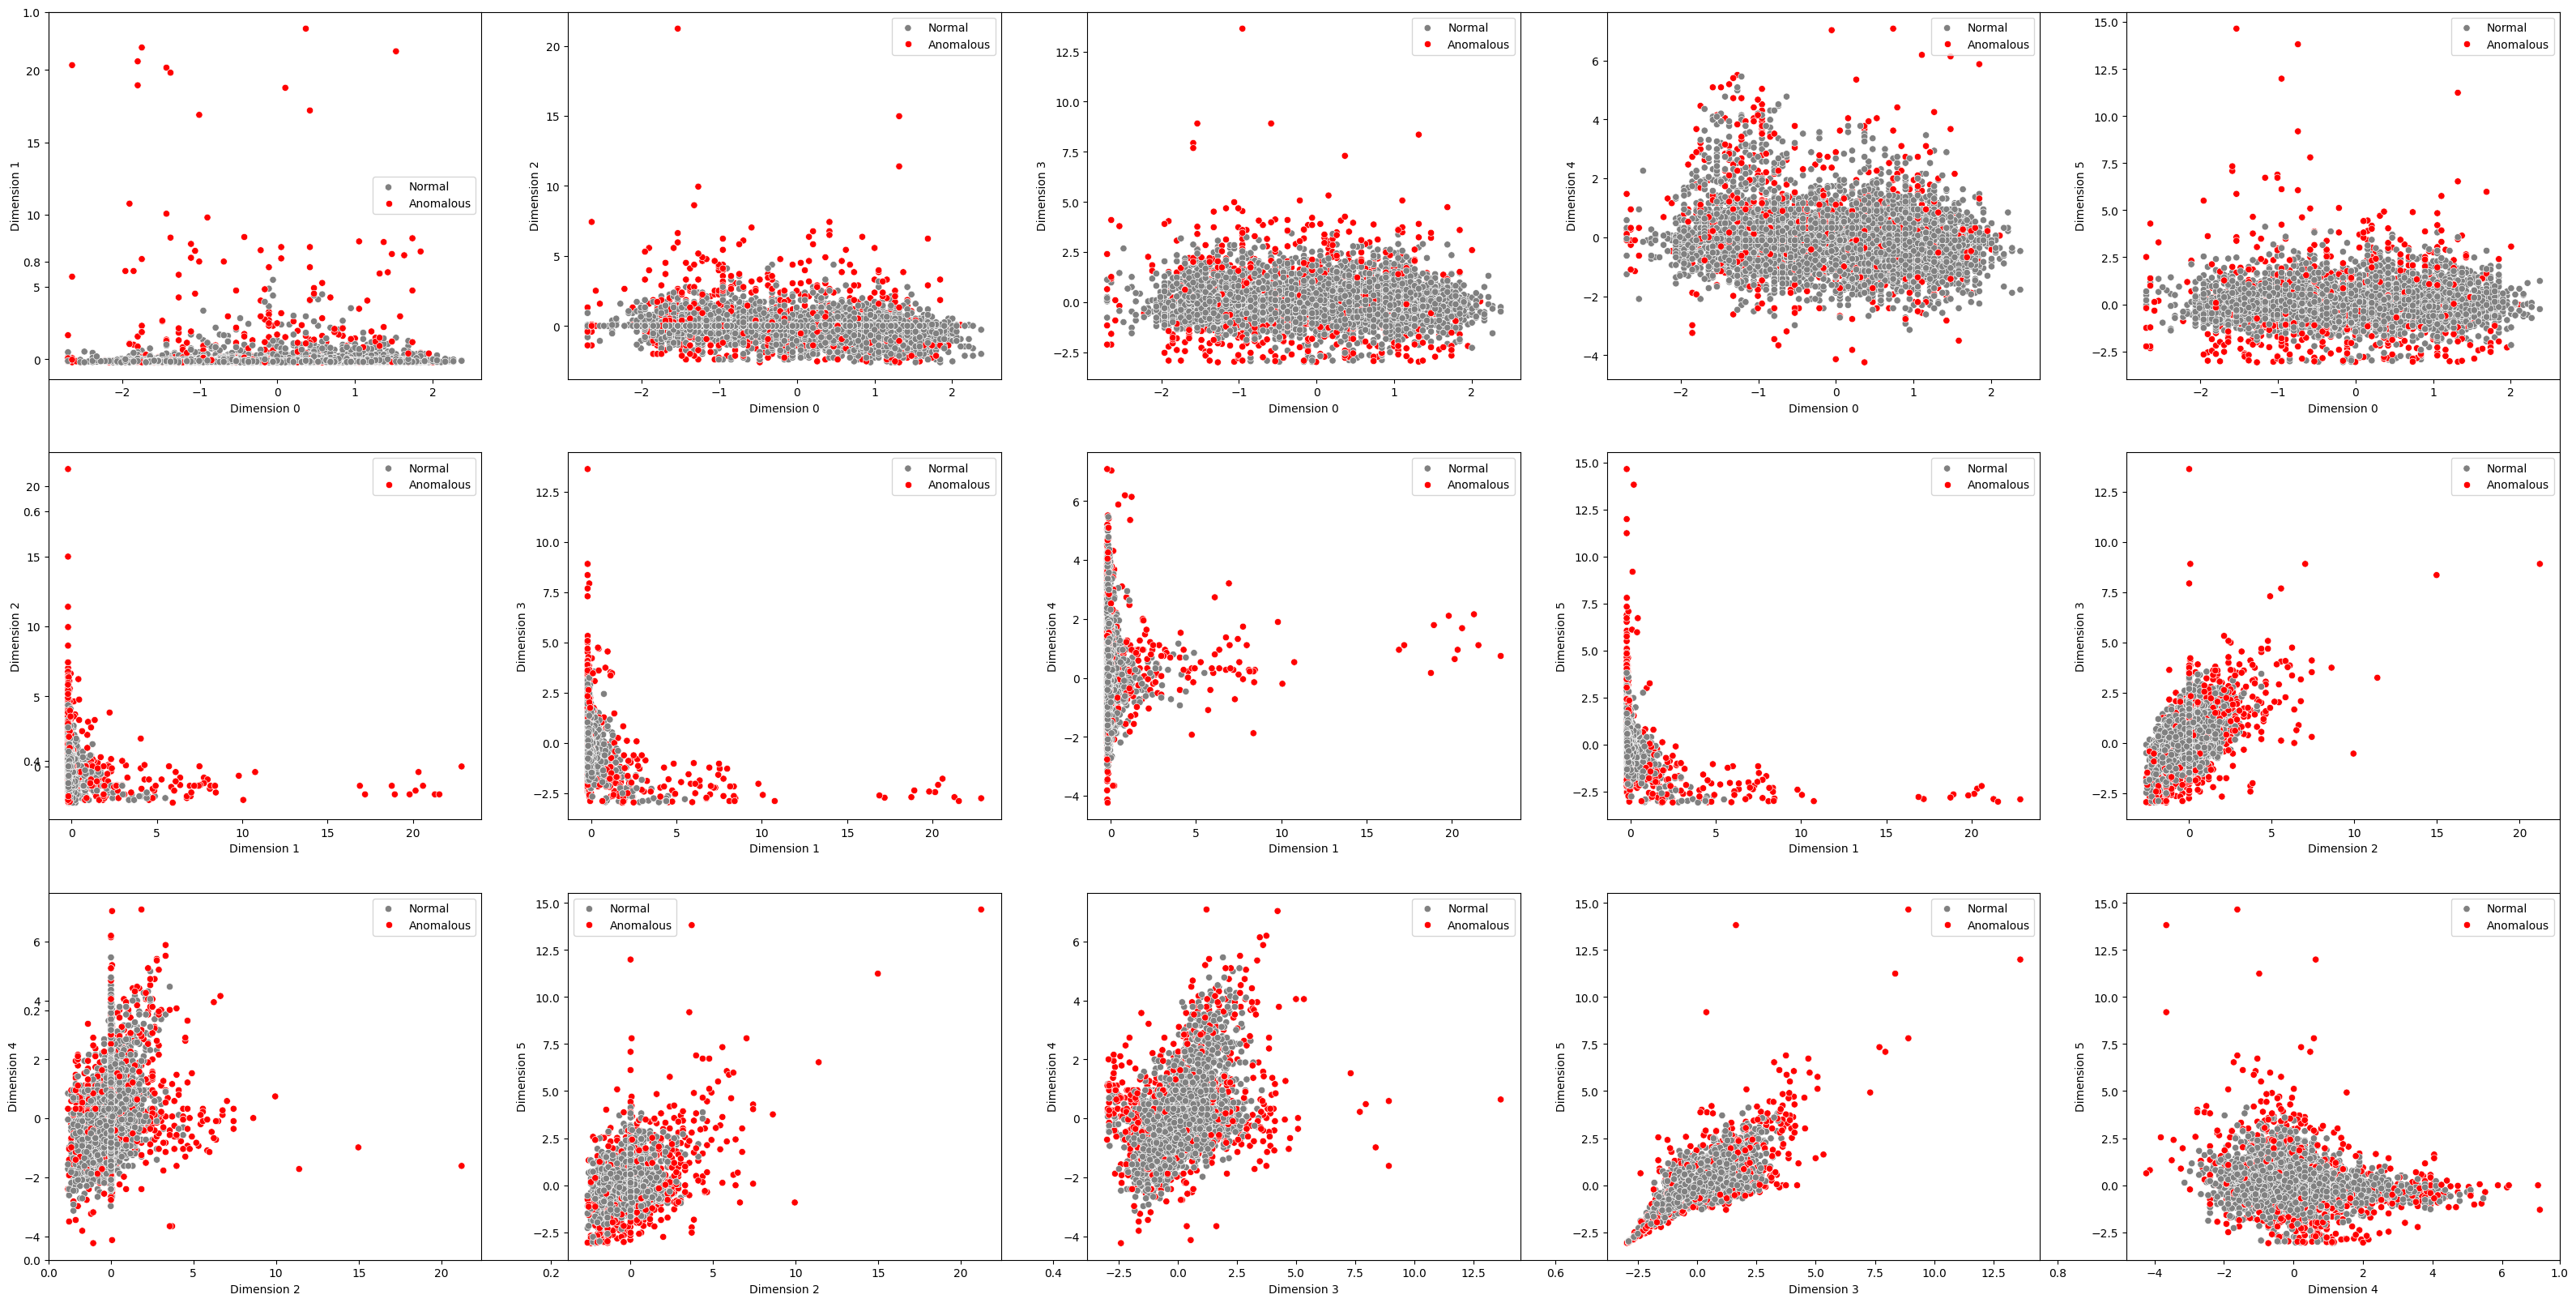
\includegraphics[width=0.80\textwidth]{images/NN_floatdims.png}
    \caption{Visual inspection of NN results on all the combinations of numerical dimensions of the data.}
    \label{fig:nn_alldims}
 \end{figure*}

\subsection{Density-based anomaly detection}
As mentioned before, density-based approaches define an anomaly if it resides in a ``low-density'' region. The notion of density is typically defined by the number of instances within a specified radius or distance threshold. This approaches tend to be particularly useful when the structure of the dataset is complex. We will now discuss the implemented density-based approached and their performances.

\subsubsection{Local Outlier Factor (LOF)}
The Local Outlier Factor (LOF) is a density-based method that assigns an outlier score to each data object based on the density of its local neighborhood compared to the densities of its neighbors. Data objects with higher LOF scores are considered more anomalous. Unfortunately, this approach is extremely sensitive to high dimensionality, a problem that we encountered in our dataset. In high-dimensional spaces, the distances between data objects tend to become similar, meaning that the difference between the nearest neighbor and the furthest neighbor decreases, making it difficult to distinguish normal data objects from anomalous ones. Another issue that arises with high dimensionality, which LOF suffers from and manifested in our case, is the sparsity introduced by the increasing number of dimensions. High-dimensional spaces are inherently sparse due to the exponential expansion of the space's volume with each added dimension, while the cardinality of the data remains the same. This sparsity causes data objects to be very far from one another, leading to very high LOF scores for many points, making it challenging to identify true outliers. As a matter of fact our LOF scores ranged between $0.8$ and $1.5\cdot 10^8$.
Indeed, by inspecting the data reduced to two dimensions through PCA and t-SNE in Figure \ref{fig:lof_pcatsne}, it is evident that the LOF detection did not mark many apparent anomalous data objects, although it marked 12.68\% of the data as anomalies, indicating numerous false positive towards the center of the mass, highlighting the limitations we faced due to the curse of dimensionality.

 \begin{figure}[h]
    \centering
    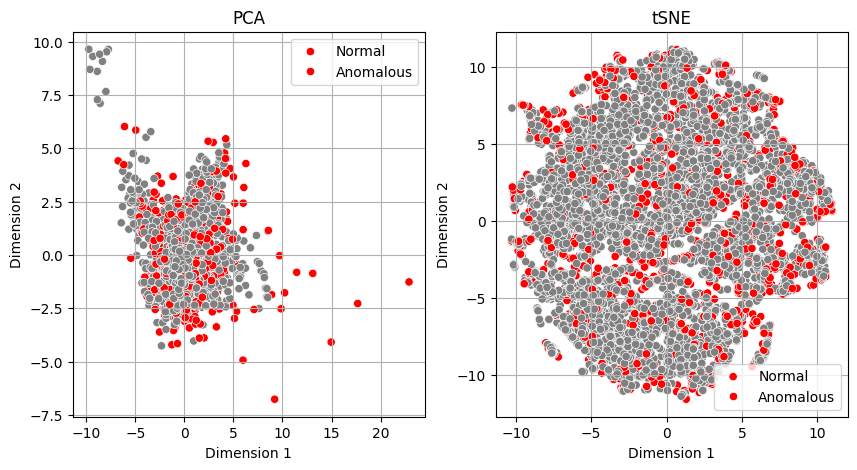
\includegraphics[width=0.5\textwidth]{images/LOF_PCATSNE.png}
    \caption{Visual inspection of LOF results on data reduced to two components.}
    \label{fig:lof_pcatsne}
 \end{figure}

\subsubsection{Connectivity Outlier Factor (COF)} % tbh this is graph-based but whatever
The Connectivity Outlier Factor (COF) is a graph-based variant of the LOF method that considers the connectivity of instances within their neighborhoods. It constructs a graph from the data, where the edges are weighted by the distances between data objects. This approach defines anomalous data objects as those that are, on average, harder to reach through their shortest paths in the graph.
Unlike the LOF method, the COF variation is less sensitive to the curse of dimensionality. As a result, we obtained much better results, as illustrated in Figure \ref{fig:cof_pcatsne}. As last confirmation that this method provides a proper anomaly score can be obtained by analyzing the histogram of the COF score assigned to each data object shown in Figure \ref{fig:cof_scores}. As we can see the distribution of the scores is well appropriate for an anomaly score, and the two-step IQR threshold cuts 784 data objects, or 10.89\% of the data. Nonetheless, it appears not to perform greatly compared to other approaches, as it is clear from Figure \ref{fig:cof_pcatsne} that there are still a significant amount of apparent false positives and false negatives.
\begin{figure}[h]
    \centering
    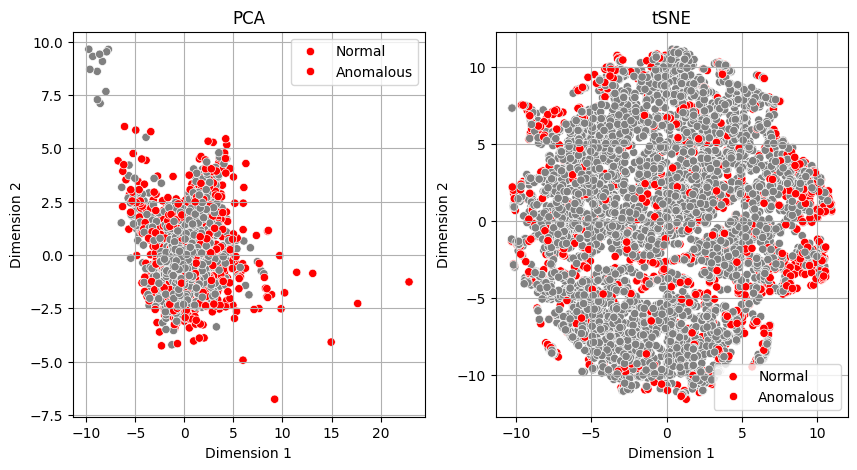
\includegraphics[width=0.5\textwidth]{images/COF_PCATSNE.png}
    \caption{Visual inspection of COF results on data reduced to two components.}
    \label{fig:cof_pcatsne}
\end{figure}

\begin{figure}[h]
    \centering
    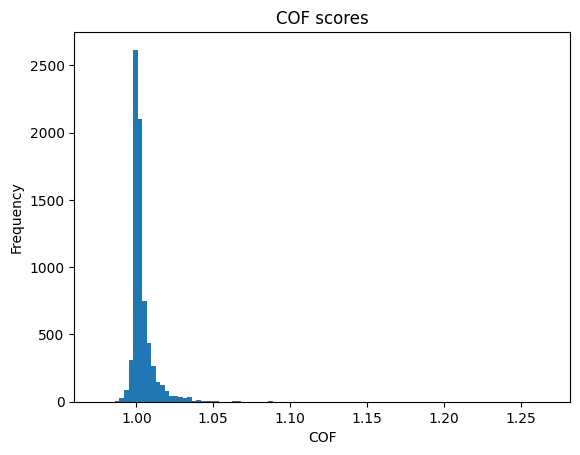
\includegraphics[width=0.5\textwidth]{images/COF_scorehist.png}
    \caption{Histogram of the COF scores of each data object.}
    \label{fig:cof_scores}
 \end{figure}
\subsubsection{DBSCAN}
While not explicitly designed for anomaly detection, the DBSCAN (Density-Based Spatial Clustering of Applications with Noise) algorithm can be adapted for this purpose. DBSCAN groups dense regions into clusters and identifies low-density instances as noise or anomalies. We are only interested to the labeling of the noise points, as those are considered anomalies by design. With a proper adjustment of the parameter, we found that an \texttt{eps} value of $0.125$ markS 4.62\% of the data as anomalies, which is an appropriate assumption for our task. By analyzing the identified anomalies in Figure \ref{fig:dbscan_pcatsne} we can distinguish very promising result. A further analysis of the combinations of numerical features suggests us that this approach appropriately marked as anomalies those points that are outliers in many dimensions.
\begin{figure}[h]
    \centering
    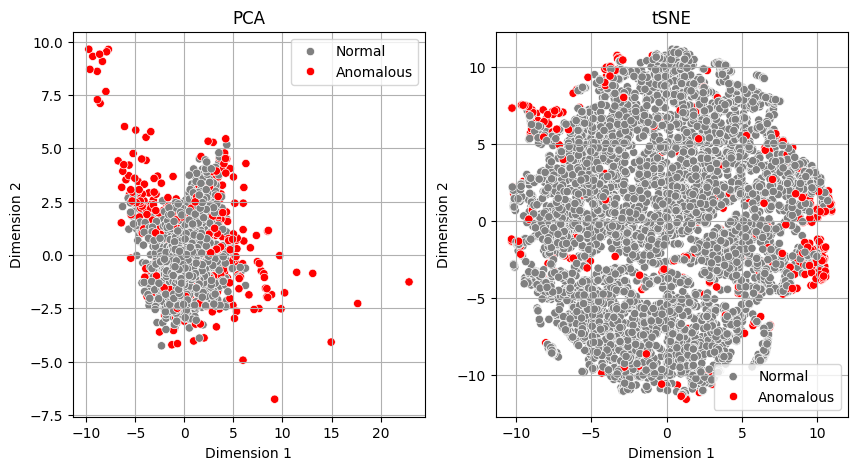
\includegraphics[width=0.5\textwidth]{images/DBSCAN_PCATSNE.png}
    \caption{Visual inspection of DBSCAN results on data reduced to two components.}
    \label{fig:dbscan_pcatsne}
\end{figure}

\section{Prototype-based\\anomaly detection}
Prototype-based anomaly detection is a method that relies on identifying representative samples, or prototypes, within a dates to differentiate between normal and anomalous data objects. This approach heavily leverages on clustering algorithm to establish prototypes that capture the inherent structure of the data. Comparing data object to their prototypes gives can effectively distinguish anomalous data objects from normal ones.

\subsection{Clustering approach with K-Means++}
The implementation uses K-Means++, an improved version of the K-Means algorithm \cite{hartigan1979algorithm}, which selects initial centroids in a way that maximizes their spread across the dataset \cite{arthur2007k}. This is done through a probabilistic process that favors points farther away from already chosen centroids. After initialization, the standard K-Means iterative process is applied:
\begin{enumerate}
    \item Assign each data point to the nearest centroid.
    \item Recalculate the centroids as the mean distance of the data objects assigned to their centroid.
    \item Repeat steps 1 and 2 until convergence, typically when the assignments no longer change or the reduction in variance falls below a threshold.
\end{enumerate}

The current downside is that available implementations of K-Means and K-Means++ in various libraries do not allow the use of multiple distances. As a result, the boolean features of the medoids (prototypes) would be represented as floating-point numbers, leading to a loss of information.

\subsection{Adapting K-means with gower distance}
To preserve the most information during computations, three things are desired: the structure of the medoid should properly represent a data object, with boolean features represented as booleans, not floats; the Gower distance or equivalent should be used when computing the distance between medoids and data objects; and the policy used to update a medoid should vary per feature type, with floats using a simple average and booleans taking the mode.

Now we can reimplement K-Means from scratch by taking into account our needs, but without a few observation it would be naïve to do so.

Now we want to pinpoint a few observations that arise from using the hamming distance for boolean features and the mode while updating the medoid.

For boolean features, computing the mode involves checking the "label" with the highest frequency. A shortcut can be found by considering True as 1 and False as 0, then
\begin{equation*}
\small
    \forall i \in \mathrm{BoolFeats} \quad \frac{1}{\vert \mathrm{data} \vert}\sum_{\mathrm{point}\in\mathrm{data}} \mathrm{point}_i = \begin{cases} \mathrm{True} & \mathrm{if }> 0.5\\ \mathrm{False}&\mathrm{else}\end{cases}
\end{equation*}

If the boolean features were treated as floats, updating the centroid would not lose information if the average were rounded to the nearest integer.
Additionally, the Hamming distance and any dissimilarity function that satisfies the condition $f(x, y) = 0 $if and only if $x = y$(such as Minkowski distance for any $p$) have the same behavior for binary values.
$$
    h(x, y) = \begin{cases}1&\mathrm{if}\; x \ne y\\ 0&\mathrm{if}\; x=y\end{cases} \\
    \forall x,y\in\{0,1\}\quad f(x, y) = \begin{cases}1&\mathrm{if}\; x \ne y\\ 0&\mathrm{if}\; x=y\end{cases}
$$ 

Based on these observations, to satisfy the requirements, K-Means can be reimplemented by treating boolean features as floats, by simply rounding the centroid's boolean representing features to the nearest integer during the update step. 

\subsection{Finding the optimal number of clusters}
Since K-Means requires the number of clusters as a hyperparameter, a study must be conducted to properly represent the data. The elbow method was used for this task. Unfortunately, the function plotting the number of clusters on the x-axis and the inertia (the sum of squared distances of samples to their closest cluster center) given by running the algorithm with x clusters has a shallow and fluctuating descent, as shown in Figure \ref{fig:elbow-method}. The shallowness of the descent is likely due to the data distribution, which cannot be changed. However, the fluctuation is caused by the variation of the K-Means algorithm due to the rounding of boolean features.
To address the fluctuation, the law of large numbers is exploited. The aim is to find a definition of the elbow point, run the elbow method several times, and choose the elbow point with the highest frequency as the optimal number of clusters.
By observing any elbow point, it is noticed that the "elbow" characterizes the point where the function "decelerates" the most. This behavior is properly captured by the second derivative, and thus the elbow point can be defined as the point where the second derivative is the lowest.
After running the elbow method several times, the optimal number of clusters is found to be around 5-6, as shown in Figure \ref{fig:opt-k-hist}.

\begin{figure}[h]
    \centering
    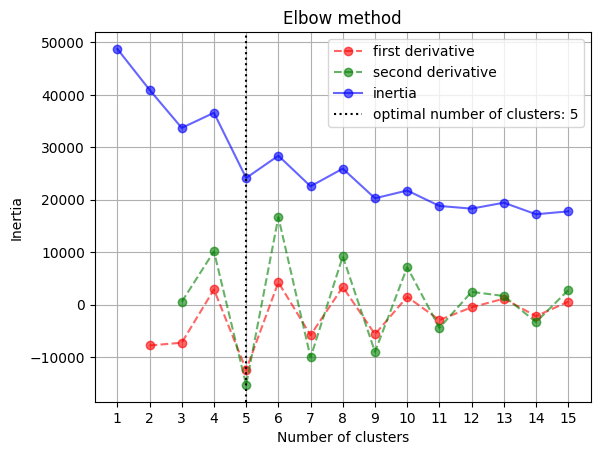
\includegraphics[width=0.5\textwidth]{images/KM_elbowmethod.png}
    \caption{Elbow method of the inertia over the number of cluster used in our variation of K-Means.}
    \label{fig:elbow-method}
\end{figure}

\begin{figure}[h]
    \centering
    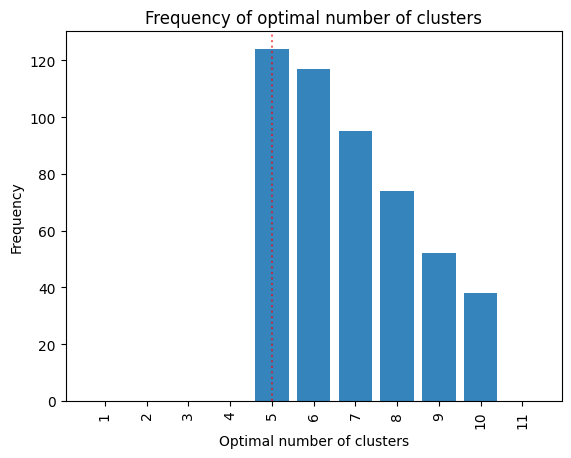
\includegraphics[width=0.5\textwidth]{images/KM_kopthist.png}
    \caption{Histogram of the optimal number of clusters (elbow point) extracted by running the elbow method 500 times.}
    \label{fig:opt-k-hist}
\end{figure}

\subsection{Investigating on outliers}
The variation of K-Means is run, and the distances of each data object to their associated medoid are extracted. A first inspection of the distribution of these distances, shown in the histogram in Figure \ref{fig:kmeans-dist-hist}, suggests that it can be used as a proper anomaly score. The two-step IQR threshold excluded 505 data objects, 7.01\% of the data.
By analyzing the data reduced to two components via PCA and t-SNE (Figure \ref{fig:kmeans_pcatsne}), it can be seen that the approach excluded the most distant point from the main mass. As already previously performed, by inspecting the combinations of numerical features (Figure \ref{fig:kmeans_floatdims}), it can be observed that this approach excluded the outer layer of each combination of dimensions, suggesting this as one of the best methods applied so far.

\begin{figure}[h]
    \centering
    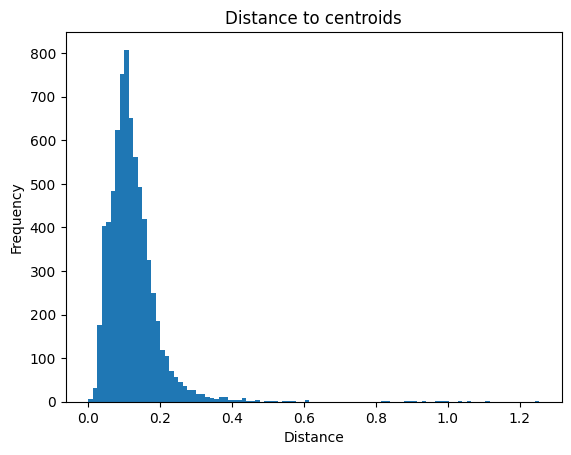
\includegraphics[width=0.5\textwidth]{images/KM_disthist.png}
    \caption{Histogram of the distances of each data object to its medoid.}
    \label{fig:kmeans-dist-hist}
\end{figure}

\begin{figure}[h]
    \centering
    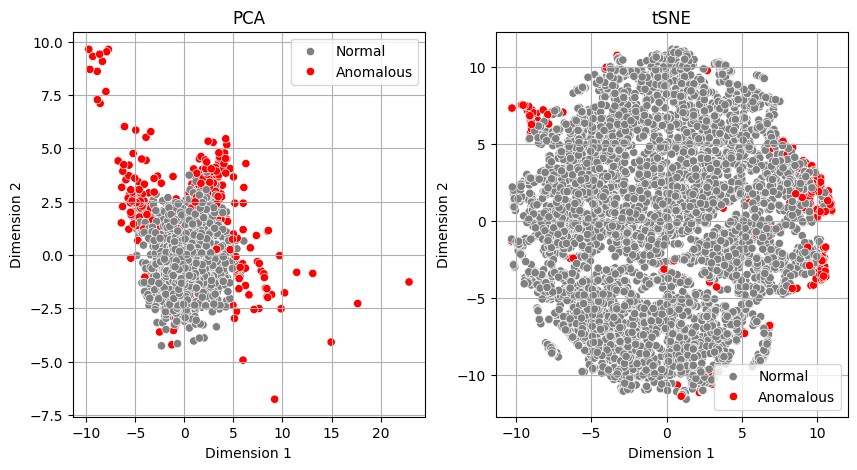
\includegraphics[width=0.5\textwidth]{images/KM_PCATSNE.png}
    \caption{Visual inspection of kmeans results on data reduced to two components.}
    \label{fig:kmeans_pcatsne}
\end{figure}

\begin{figure*}[h]
    \centering
    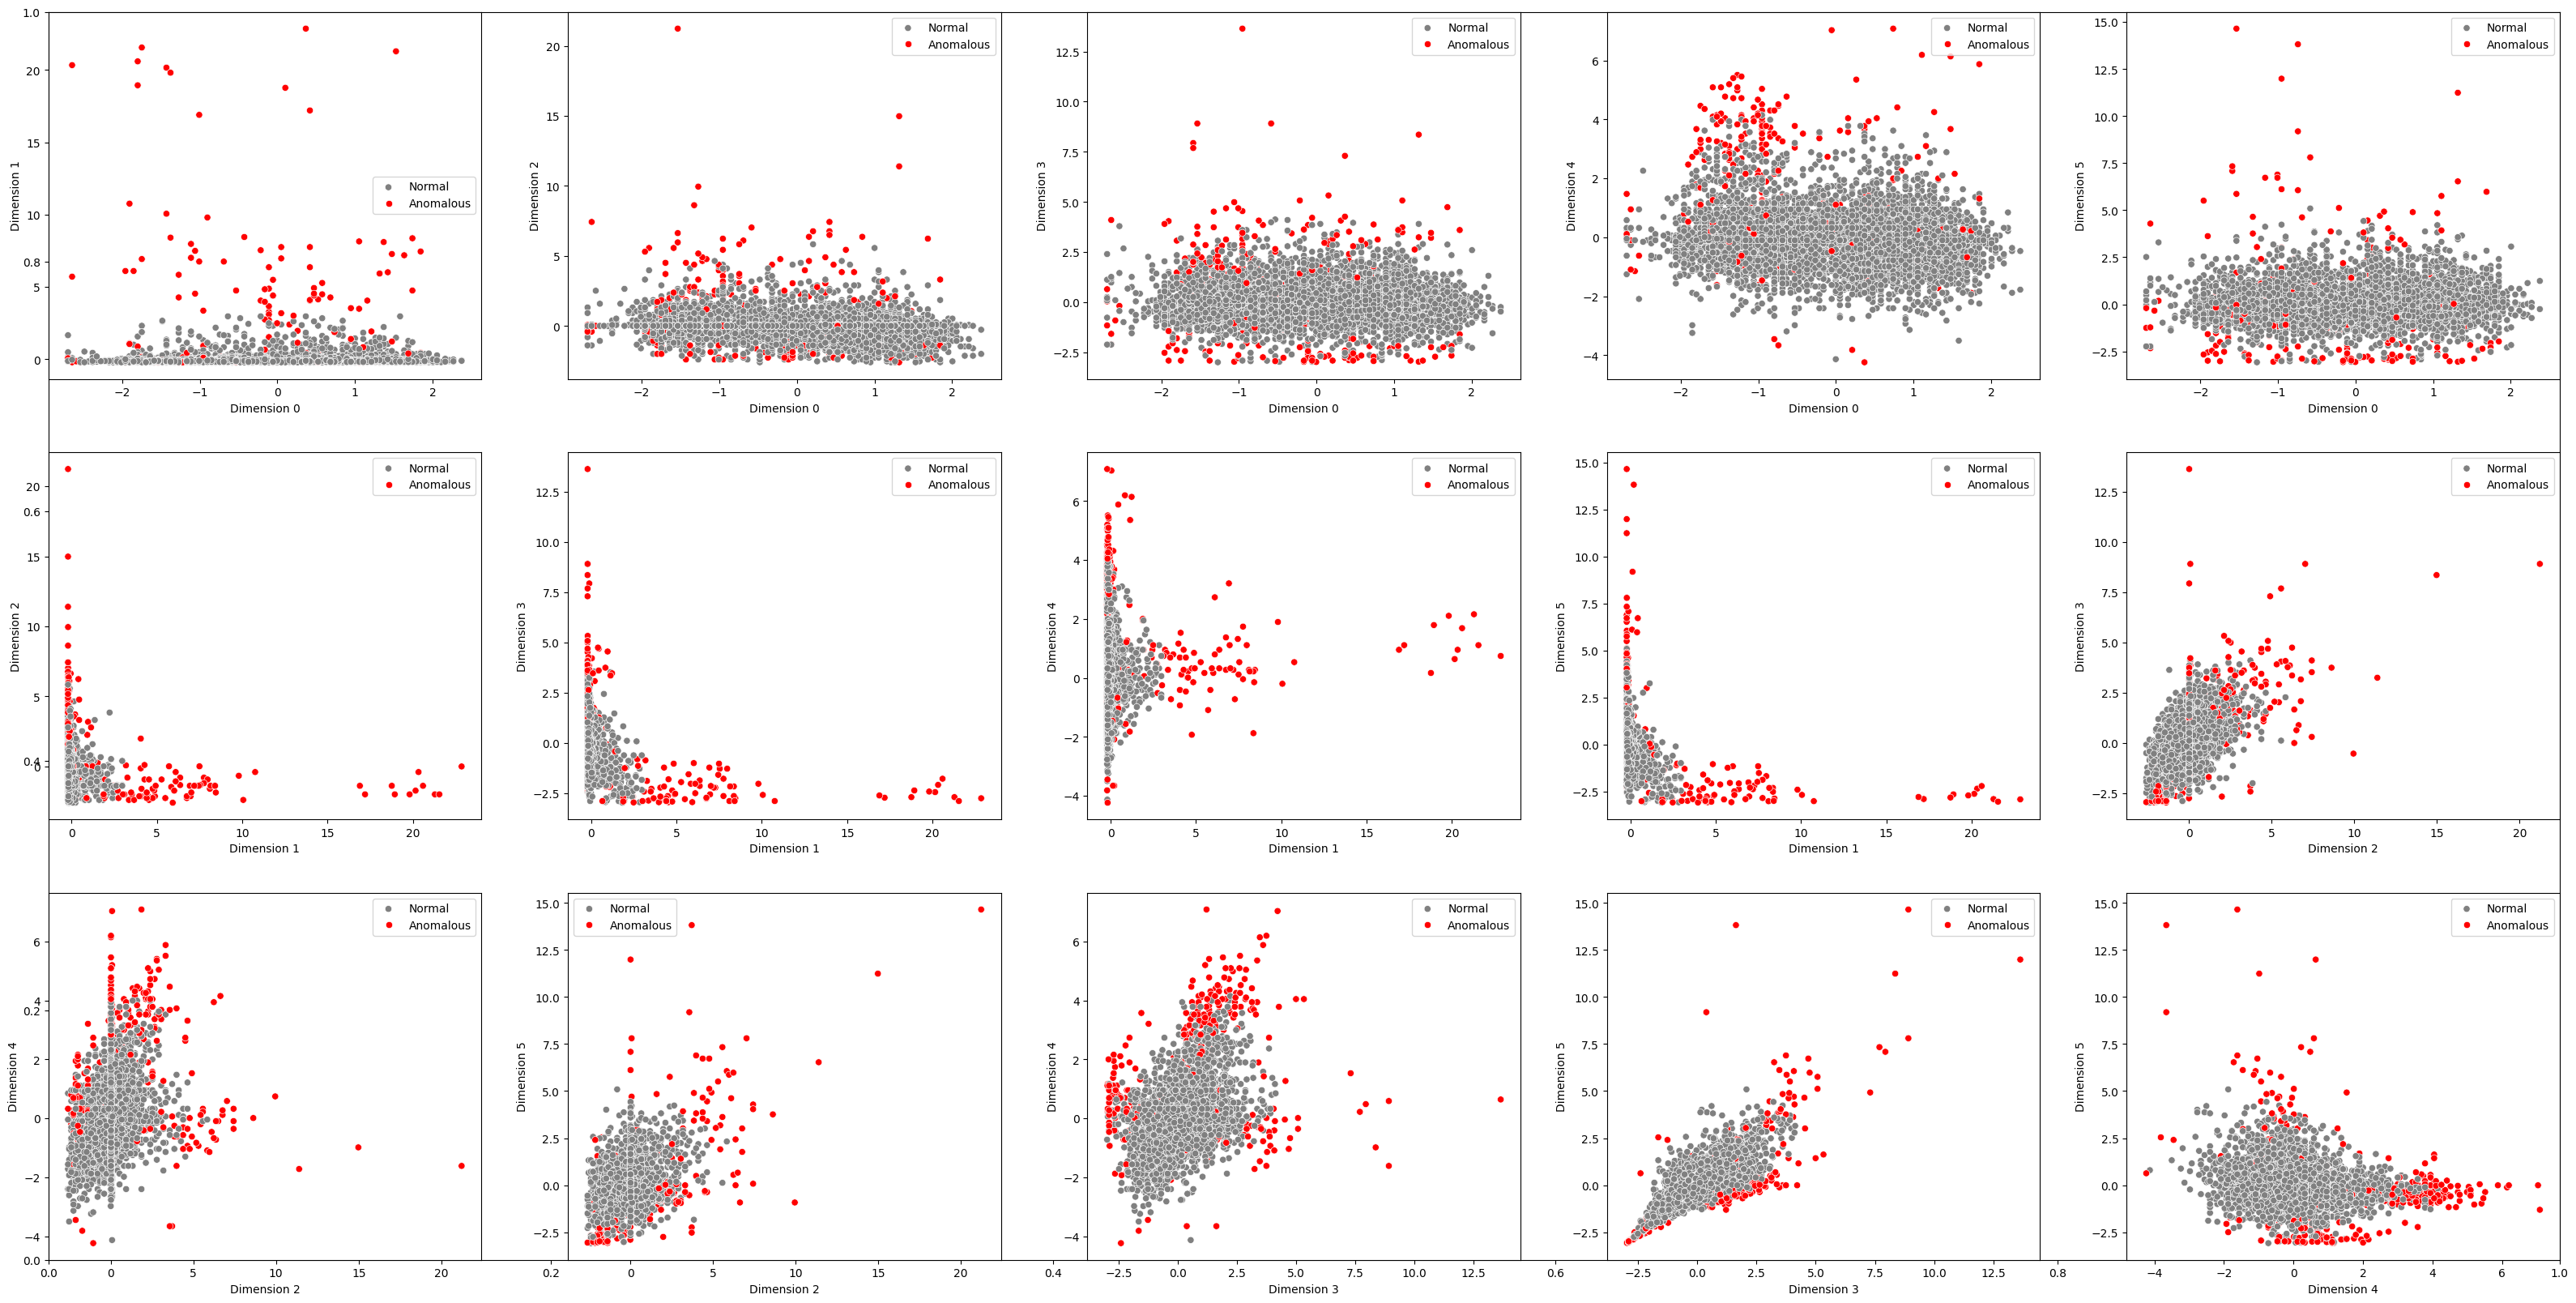
\includegraphics[width=0.80\textwidth]{images/KM_floatdims.png}
    \caption{Visual inspection of kmeans results on all the combinations of numerical dimensions of the data.}
    \label{fig:kmeans_floatdims}
\end{figure*}


\section{Reconstruction-based\\ anomaly detection}

Reconstruction-based anomaly detection methods aim to identify anomalies by examining the extent to which a data instance can be faithfully reconstructed from a learned model of the normal data instances. These methods assume that normal data instances can be effectively reconstructed, while anomalous instances, being different from the learned model, will have higher reconstruction errors. A key advantage of reconstruction-based methods is that they can capture more complex patterns and relationships within the data, as opposed to purely distance-based methods. However, the effectiveness of these methods depends on the ability to accurately model the normal instances and the choice of the reconstruction error metric.

\subsection{Principal Component Analysis}
Principal Component Analysis (PCA) is a widely used dimensionality reduction technique, it aims to find a lower-dimensional representation of the data that captures the most significant variations while minimizing information loss. By projecting the data onto a lower-dimensional subspace defined by the principal components, PCA can effectively model the normal behavior of the data.\\
Once the PCA model has been fitted to the data, it can be used to reconstruct the original data from the reduced-dimensional representation. Anomalies are then identified by measuring the reconstruction error, which quantifies the discrepancy between the original data and its reconstructed counterpart. Data points with high reconstruction errors are considered anomalous, as they deviate significantly from the learned normal patterns.
\begin{figure}[h]
    \centering
    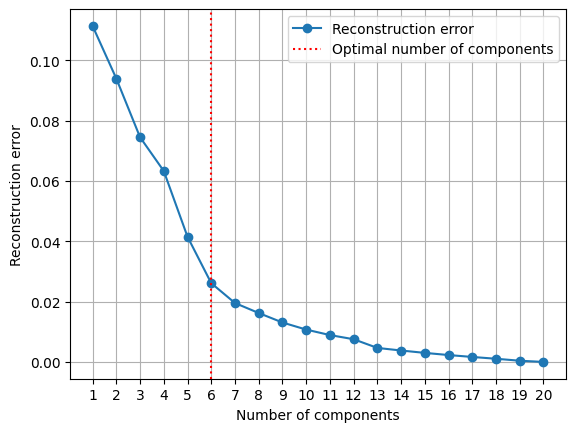
\includegraphics[width=0.5\textwidth]{images/PCA_errorelbow.png}
    \caption{reconstruction error of the PCA on the entire data with different components}
    \label{fig:pca_components}
 \end{figure}
The effectiveness of PCA for anomaly detection lies in its ability to capture the dominant patterns and variations in the data. By focusing on the most informative principal components, PCA can effectively model the normal behavior and detect anomalies that do not conform to these patterns.\\
To determine the optimal number of components, we plotted the overall reconstruction error for all data objects while varying the number of components, as shown in Figure \ref{fig:pca_components}. Our goal was to find the most representative representation with the least number of components. Based on this analysis, we selected 6 components for our PCA model. Unfortunately, by analyzing the histogram of the reconstruction error of each data point depicted in Figure \ref{fig:PCA_errorhist}, it seems that this score doesn't properly fit the usual gaussian distribution that we would like to see in an anomaly score, likely causing our threshold to mark only 1.4\% of the data, with 101 data objects. Although it still preserves the property of having few data objects with very high scores, many of the identified anomalies seems to be false positives.

\begin{figure}[h]
    \centering
    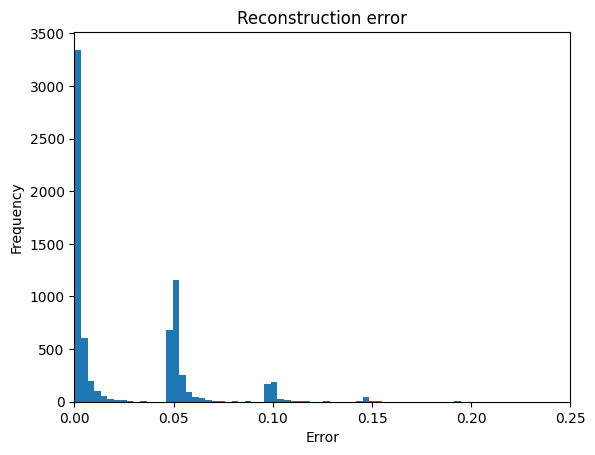
\includegraphics[width=0.5\textwidth]{images/PCA_errorhist.png}
    \caption{Visual inspection of PCA with 6 components results on data reduced to 2 components.}
    \label{fig:PCA_errorhist}
\end{figure}

\begin{figure}[h]
    \centering
    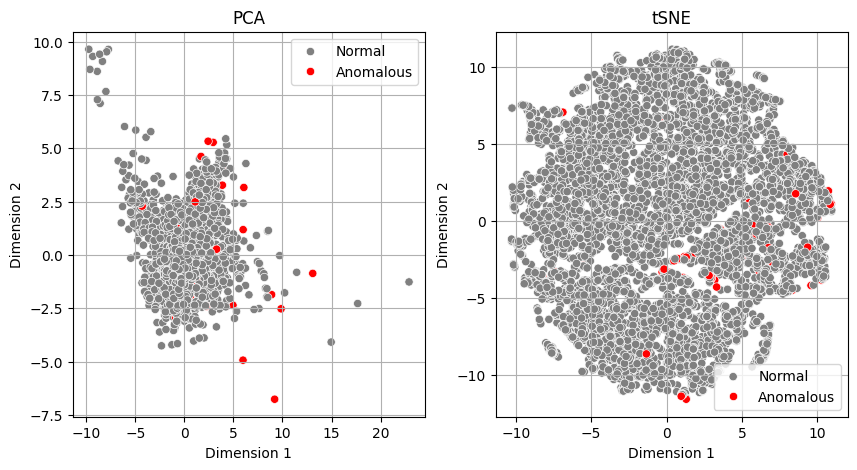
\includegraphics[width=0.5\textwidth]{images/PCA_PCATSNE.png}
    \caption{Visual inspection of PCA with 6 components results on data reduced to 2 components.}
    \label{fig:pca_pcatsne}
\end{figure}

Figure \ref{fig:pca_pcatsne} illustrates the results of applying PCA for anomaly detection on our dataset. While the PCA approach correctly identified some anomalies, it also successfully reconstructed apparent anomalous data. Suggesting that PCA may not be the most suitable technique for our specific anomaly detection task, as it struggles to differentiate between true anomalies and outliers that can be well-reconstructed by the model.

\subsection {Encoder-Decoder}
Encoder-Decoder networks, also known as autoencoders, are neural network architectures consisting of two main components: an encoder and a decoder. The encoder learns a compressed representation (encoding) of the input data, while the decoder aims to reconstruct the original data from the compressed representation. They offer a powerful mean to capture complex, non-linear relationships in the data and learn meaningful representations

In the context of anomaly detection, Encoder-Decoder networks are trained on normal data to minimize the reconstruction error. By learning to effectively reconstruct normal instances, the network captures the underlying patterns and structures present in the data. Anomalies, which deviate from these learned patterns, typically result in higher reconstruction errors compared to normal instances.
The network learns to minimize the discrepancy between the original data and its reconstructed version.

For our task, the encoder consisted of a linear layer with an input dimension of 21 nodes and a ReLU activation function, while the decoder comprised a linear layer with 6 input nodes (from the encoder) and a sigmoid activation function. The network was trained for 100 epochs, which took approximately 1.5 minutes on a high-end consumer processor.

Through the two-step IQR thresholding we found 350 anomalies, or 4.86\% of the data. By inspecting the anomalies detected (Figure \ref{fig:autoencoders_PCATSNE} and \ref{fig:autoencoders_alldims}), it is evident that the Encoder-Decoder approach effectively captures abnormal data objects, yielding results similar to the k-NN method. 

\begin{figure}[h]
    \centering
    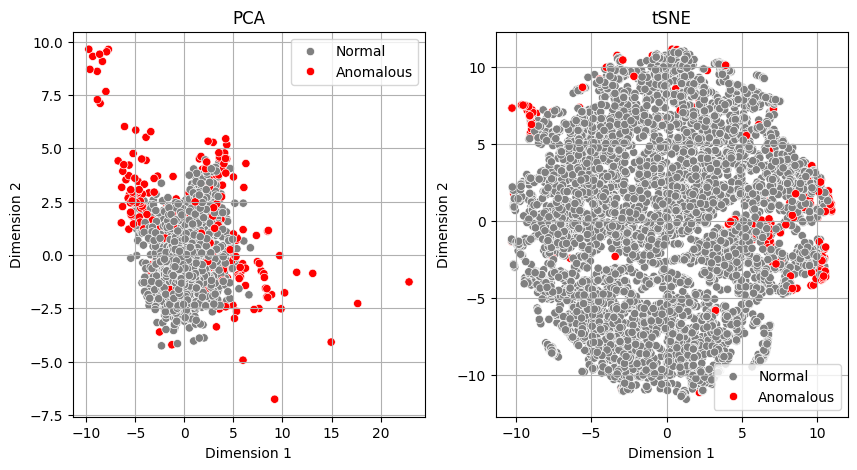
\includegraphics[width=0.5\textwidth]{images/ED_PCATSNE.png}
    \caption{Visual inspection of autoencoders results on data reduced to two components.}
    \label{fig:autoencoders_PCATSNE}
\end{figure}

\begin{figure*}[h]
    \centering
    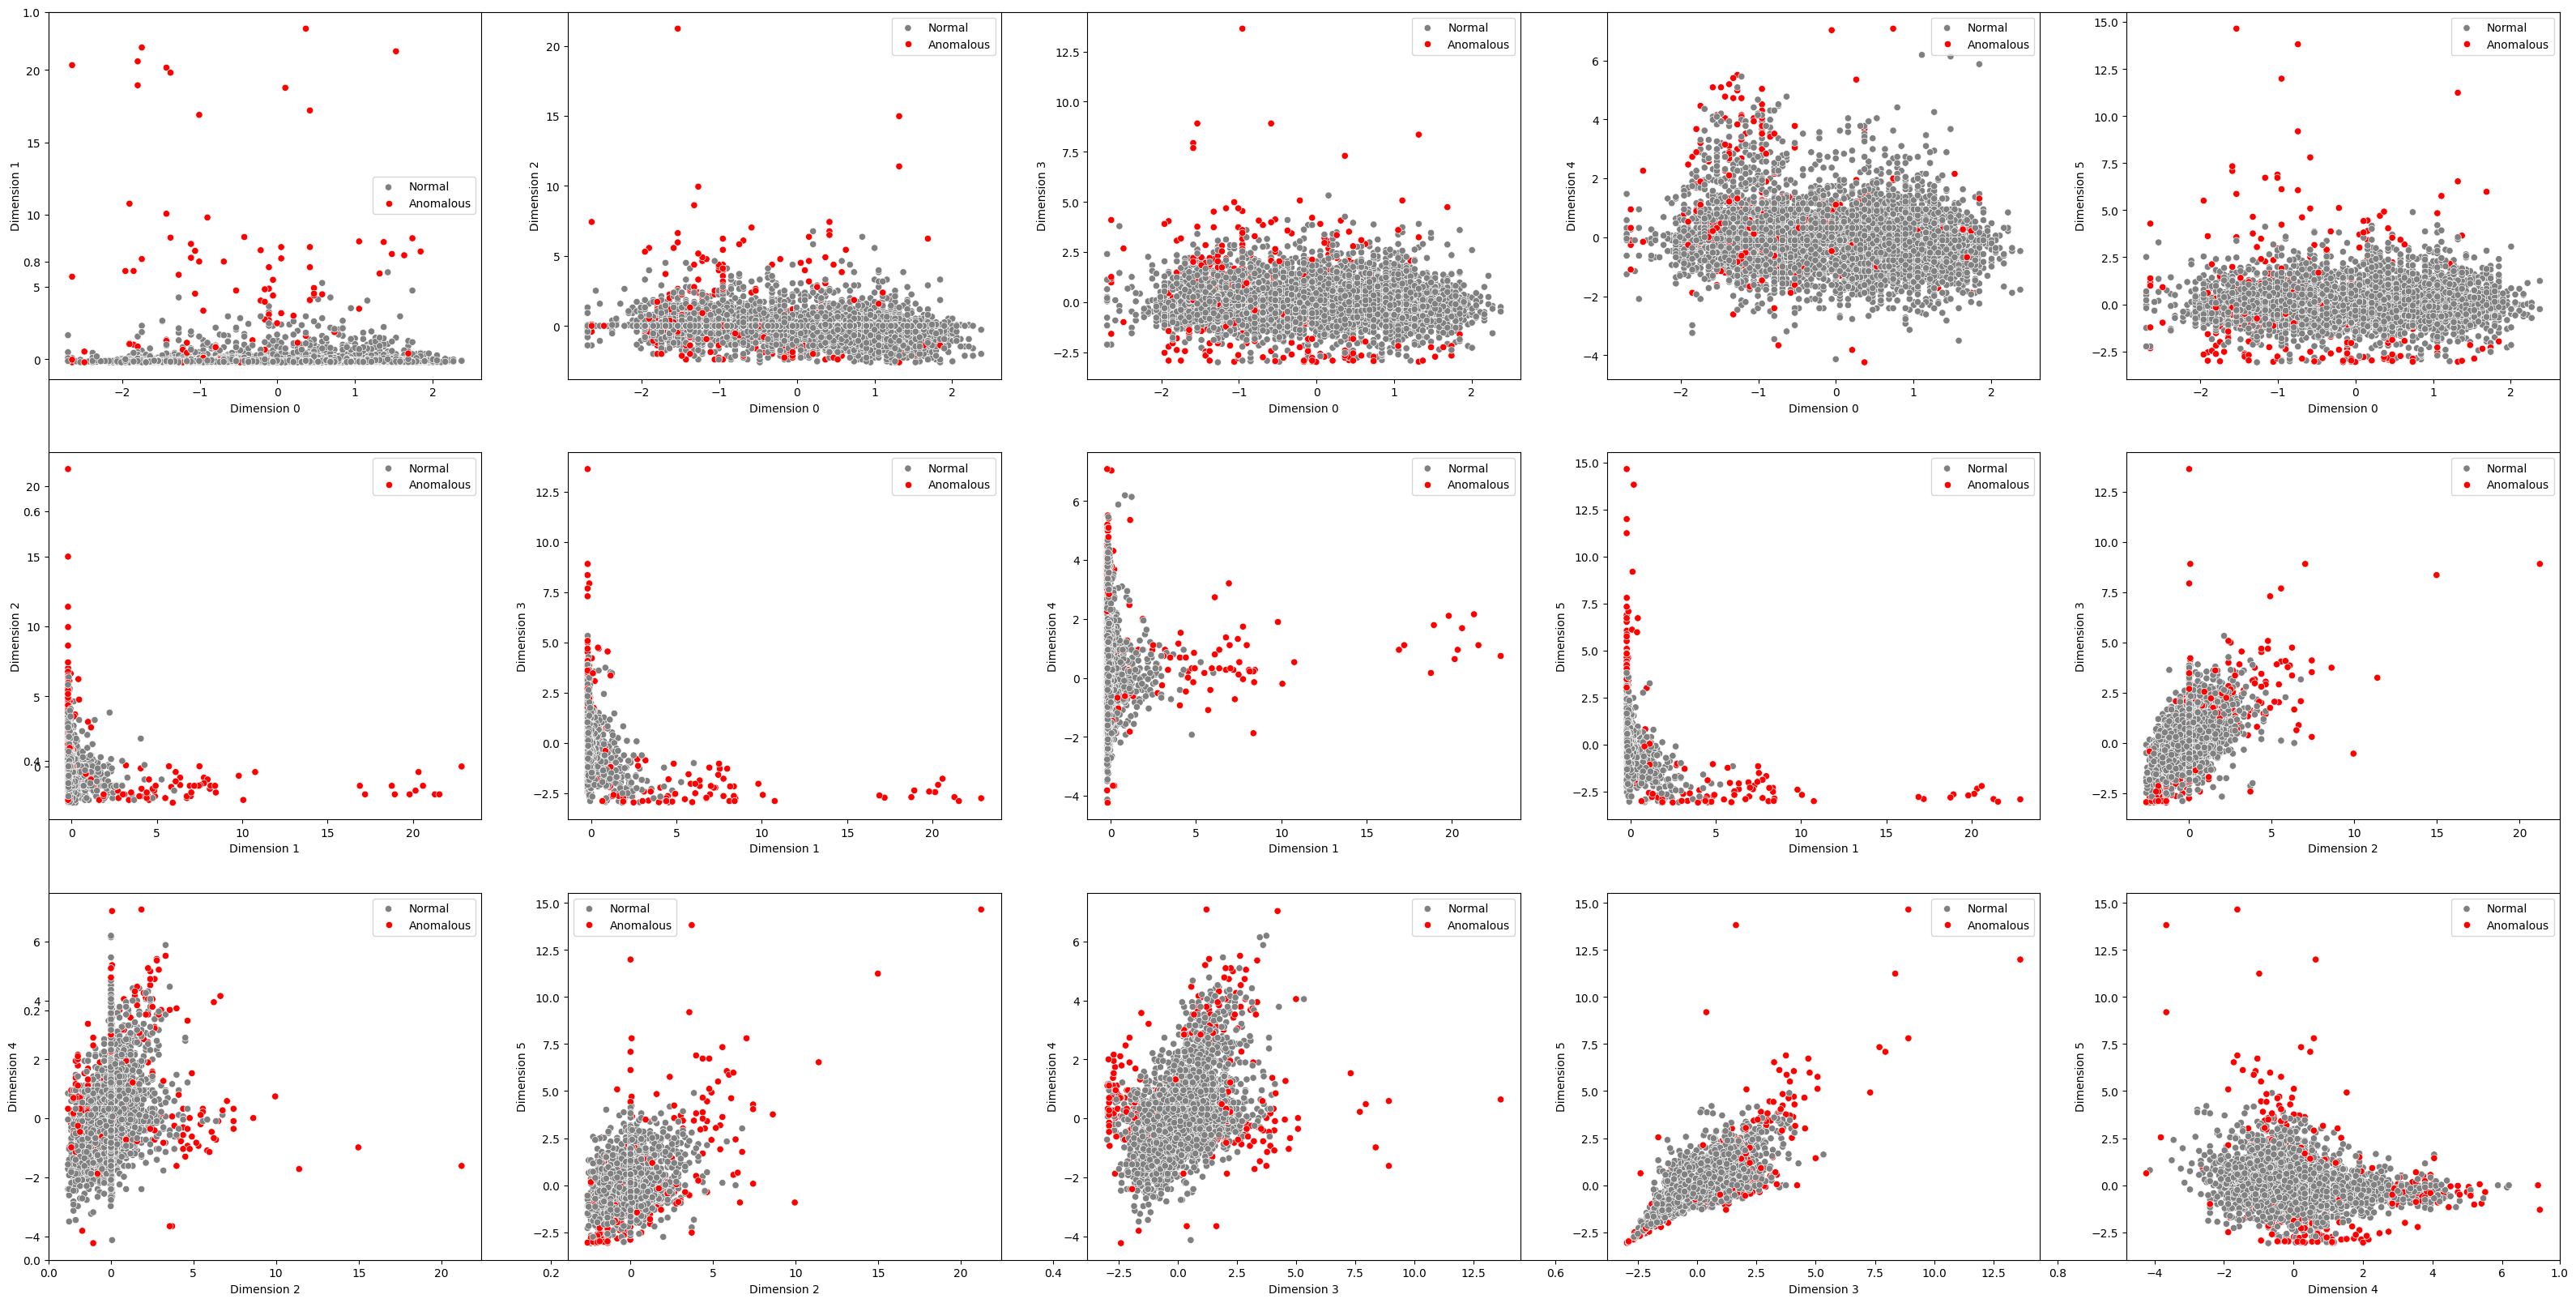
\includegraphics[width=0.80\textwidth]{images/ED_floatdims.png}
    \caption{Anomaly detection results using autoencoders, visualized with all the combinations of the numerical dimensions.}
    \label{fig:autoencoders_alldims}
\end{figure*}

\section{Ensembles}
To construct a more robust and comprehensive list of anomalies, we employed an ensemble approach that combines the results from multiple anomaly detection methods. We considered three ensemble strategies: "AND", "OR" and a weighted sum.

In the "AND" ensemble, an anomaly is identified only if it is flagged as anomalous by all the considered methods. This approach focuses on the consensus among the detectors and provides a more conservative list of anomalies. This approach greatly reduces the probability of obtaining false positives at the cost of having a larger amount of false negatives. By combining our most promising methods: K-Means, autoencoders, NN and DBSCAN, obtaining 51 anomalies, or 0.71\% of the data

On the other hand, the "OR" ensemble identifies an anomaly if it is flagged as anomalous by at least one of the methods. This approach yields a wider list of potential anomalies, as it considers the union of the anomalies detected by individual methods. The "OR" ensemble aims to capture a broader range of anomalous instances, reducing false negatives, but at the expenses of potentially more false positives. We combined the same methods as above, obtaining 1347 anomalies, or 18.71\% of the data

To strike a balance in between these two methods we propose a weighted sum of methods. By taking into consideration the normalized scores of each method and performing a weighted sum, where each weight determines which method should be considered the most, we get an overall score of anomaly. The included methods are the same as before but excluding DBSCAN as we don't have a proper score for it. Since K-Means, Autoencoders and NN seems to be equally promising, an equal weight is assigned to each, and after thresholding a total of 545 anomalies are found, or 7.57\% of the data. As shown in Figure 

\begin{figure*}[h]
    \centering
    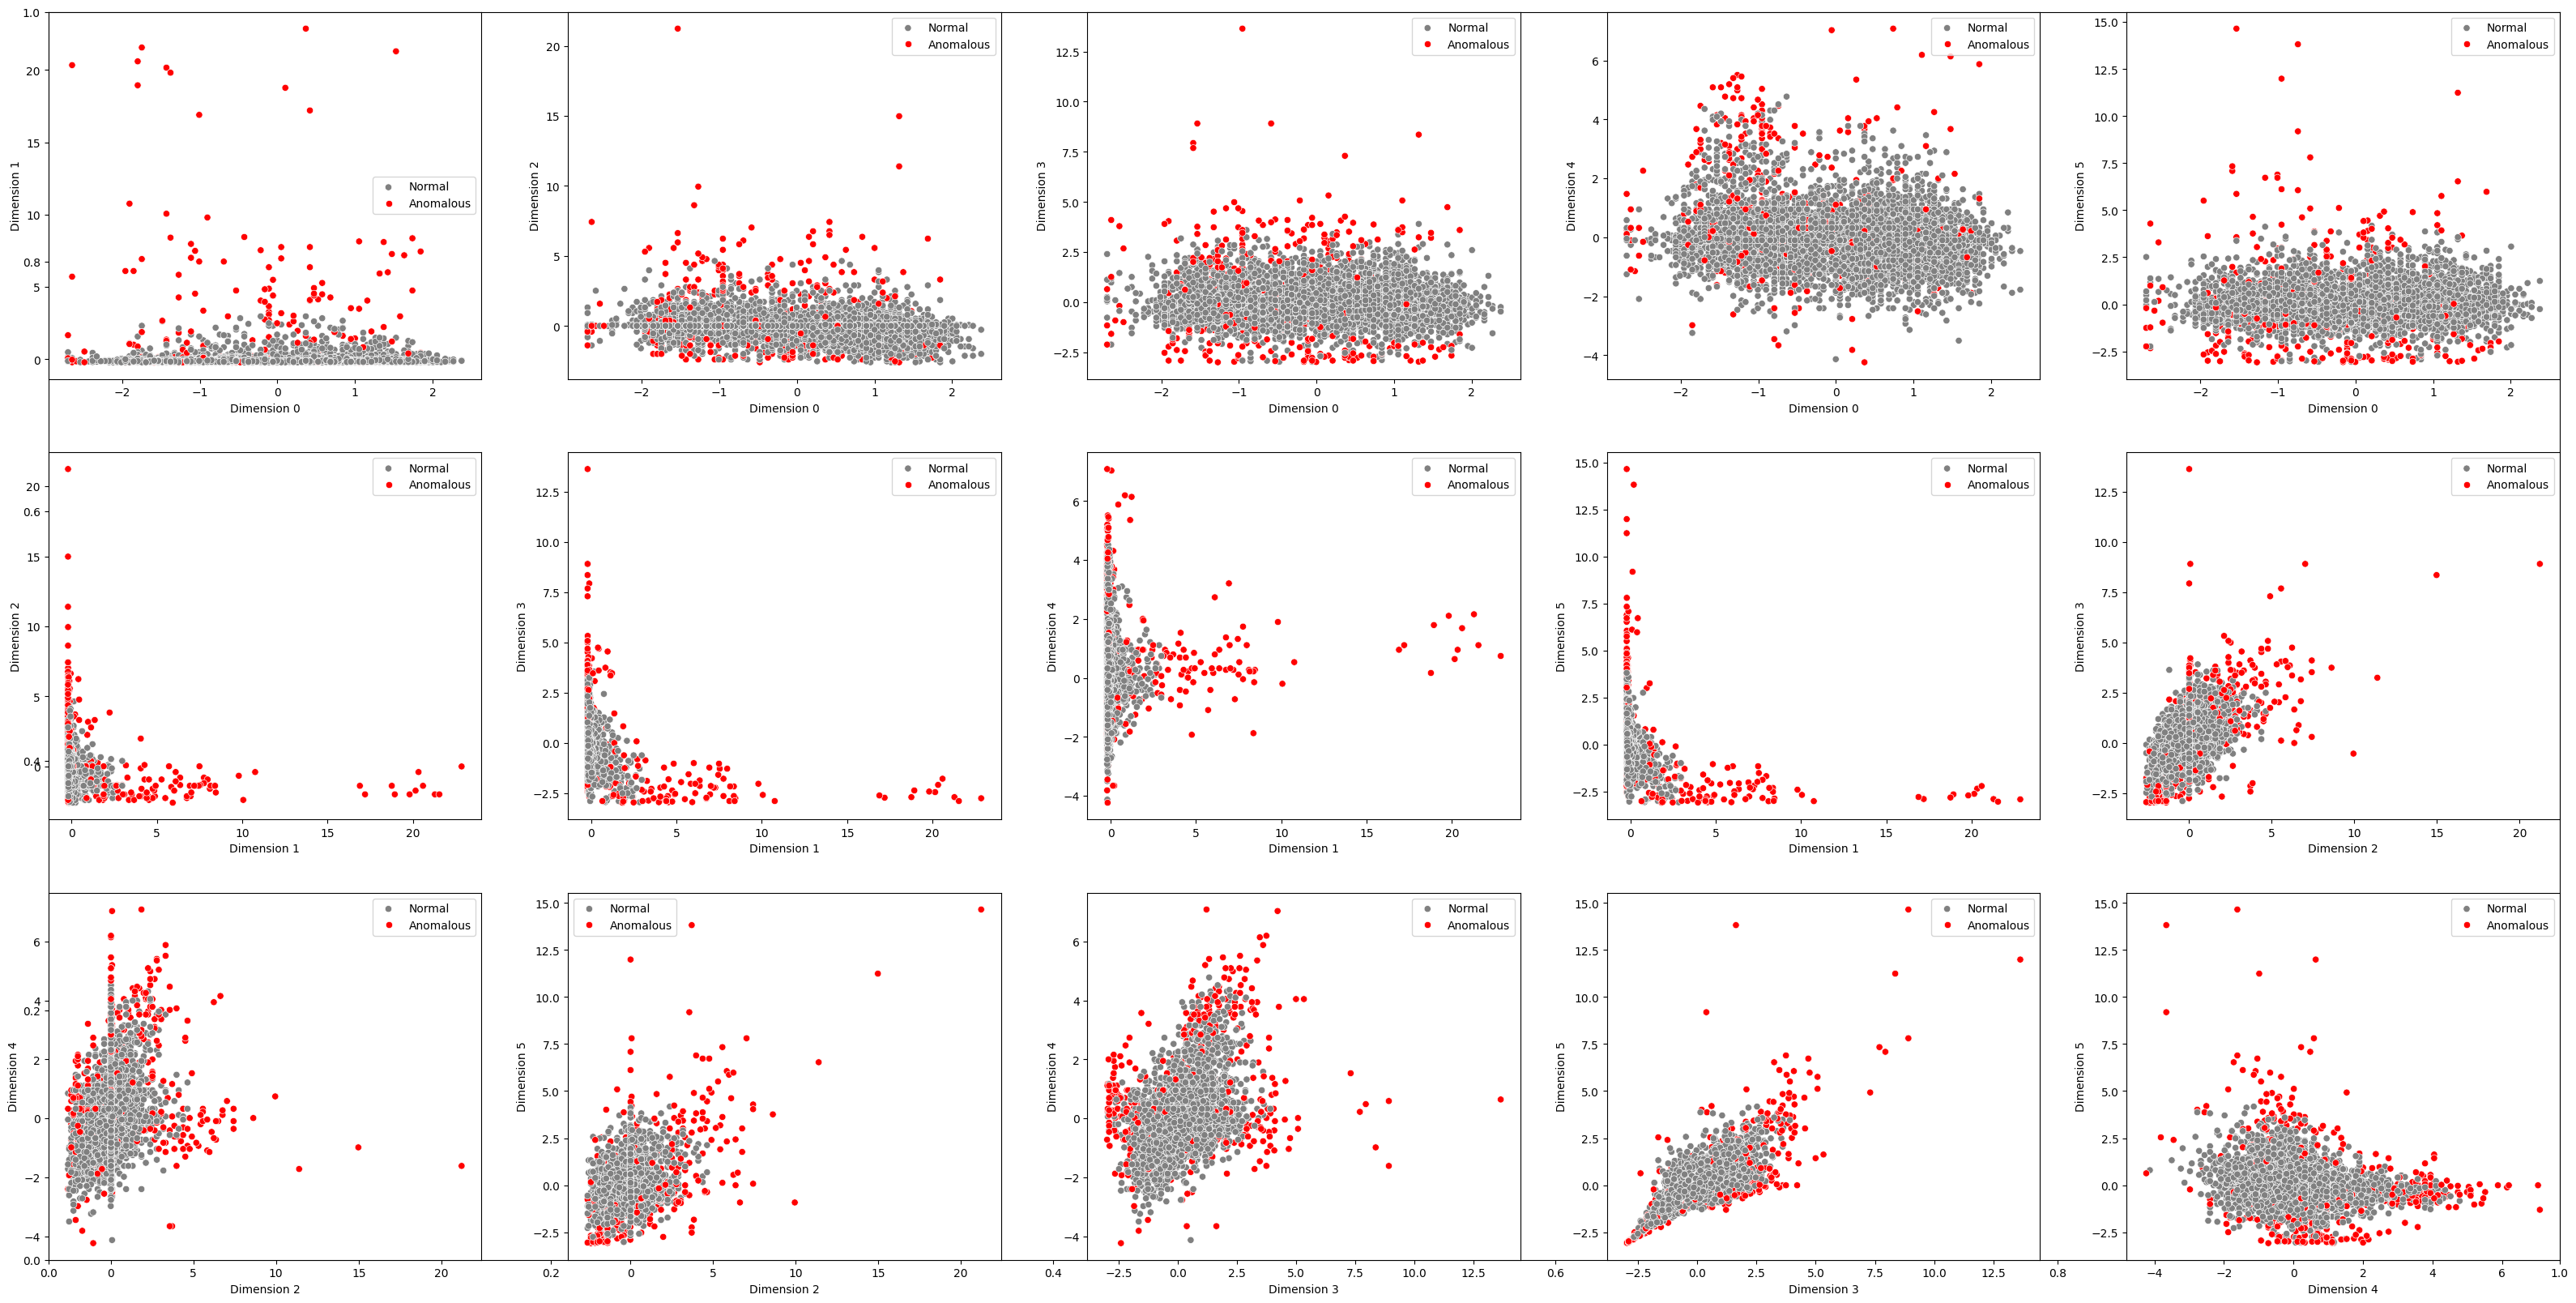
\includegraphics[width=0.80\textwidth]{images/WS_floatdims.png}
    \caption{Anomaly detection results using a weighted sum (with uniform weights) of K-Means, Autoencoders and NN visualized with all the combinations of the numerical dimensions.}
    \label{fig:autoencoders_alldims}
\end{figure*}

\section{Coherence between detectors}
Since we proposed several approaches for anomaly detection, we expect some degree of agreement between them. To evaluate the coherence between them we adopted several metrics commonly used for clustering comparison: homogeneity, completeness, V-measure, Rand index adjusted for chance, and adjusted mutual information.
In this report we will focus on the Rand index adjusted in order to briefly show that methods that we referred to as ''promising`` tend to agree with each other up to a certain degree, while for expected ''low performance`` methods we'll see a very low degree of agreement with others.

The adjusted Rand index quantifies the similarity between two anomaly detection results, considering both true positives and true negatives. It ranges from -1 to 1, with higher values indicating better agreement between the methods.

\begin{table}[h]
    \centering
    \small
    \begin{adjustbox}{max width=.63\textwidth}
    \begin{tabular}{lcccccccc}
        & NN & LOF & COF & DBSCAN & K-Means & Autoenc. & PCA & W. sum \\
        \hline
        NN & 1.0000 & 0.1333 & 0.4089 & 0.8038 & 0.5913 & 0.5495 & 0.2292 & 0.6896 \\
        LOF & 0.1333 & 1.0000 & 0.2408 & 0.1509 & 0.0274 & 0.0307 & 0.0999 & 0.0591 \\
        COF & 0.4089 & 0.2408 & 1.0000 & 0.3369 & 0.2795 & 0.2345 & 0.1395 & 0.3508 \\
        DBSCAN & 0.8038 & 0.1509 & 0.3369 & 1.0000 & 0.5529 & 0.5562 & 0.2622 & 0.6150 \\
        K-Means & 0.5913 & 0.0274 & 0.2795 & 0.5529 & 1.0000 & 0.6928 & 0.1593 & 0.8278 \\
        Autoenc. & 0.5495 & 0.0307 & 0.2345 & 0.5562 & 0.6928 & 1.0000 & 0.1503 & 0.7321 \\
        PCA & 0.2292 & 0.0999 & 0.1395 & 0.2622 & 0.1593 & 0.1503 & 1.0000 & 0.1706 \\
        W. sum & 0.6896 & 0.0591 & 0.3508 & 0.6150 & 0.8278 & 0.7321 & 0.1706 & 1.0000 \\
    \end{tabular}
    \end{adjustbox}
    \caption{Comparison of different methods}
    \label{tab:comparison}
\end{table}

\section{Conclusions}
Several approaches of anomaly detection have been tested, each defining an anomaly in a different way. The most promising approach combines several of them in a single ensemble, trying to take into account patterns that are unveiled only by some of them. Due to the mixed nature of the data, particular attention has been given to the distance used within the various approaches: gower's distance (or equivalent) has been carefully applied, preserving information as best as possible during computations. According to our analysis, the amount of anomalies for this specific dataset seems to be around a reasonable 5-9\%.   

\bibliographystyle{plain}
\bibliography{bibliography/references} 
\end{document}